\documentclass{article}
\usepackage{pdfpages}
\usepackage[utf8]{inputenc}
\usepackage[english]{babel}
\usepackage{hyperref}
\usepackage{apacite}
\usepackage{mathptmx}
\usepackage[font = {small, it}]{caption}
\DeclareCaptionLabelFormat{cont}{#1~#2\alph{ContinuedFloat}}
\captionsetup[ContinuedFloat]{labelformat=cont}
\usepackage{subcaption}
\usepackage{float}
\usepackage{fancyhdr}
\usepackage{graphicx}
\usepackage{amsmath}
\setlength{\parindent}{2em}
\setlength{\parskip}{1em}
\renewcommand{\baselinestretch}{1.5}


\fancypagestyle{plain}{
\fancyhf{}
\rhead{Mikkel Werling (201706722) \\ Victor Møller Poulsen (201707639)}
\lhead{Smart homes for dummies}
\cfoot{\thepage}
}
\pagestyle{plain}

\title{Smart homes for dummies}
\author{Mikkel Werling (201706722) \\ Victor Møller Poulsen (201707639)}
\date{January 2021}

\begin{document}
    \maketitle
    REMEMBER TO FUCKING ADD THE NAMES TO THE SECTIONS 
    \section{Abstract}
    This paper uses topic modeling to investigate the debate amongst smart home users on Reddit. We find that the topics generated bottom-up match smart technology categories proposed in \citeA{hubert2020take} but that some smart home technologies are disproportionately discussed. Keywords “privacy”, “trust” and “security” were used to investigate in more detail the specific debate surrounding data privacy. It was found that this is a marginal topic, but that user’s really care about securing their homes.  
    \begin{center}
    Github: \url{https://github.com/SmartHomeNLP/SmartHomeNLP}
\end{center}

    \section{Introduction}
    \subsection{Smarthome - what's the buzz?}
    It is often stated that the world is becoming more connected. While this sentiment usually refers to the connections between people, it is also true for our devices. Devices can now share information with each other and interact seamlessly with users. Networks of communication between devices and users in private homes are generally called “smart homes” and their components are called “smart devices” \cite{novak2019relationship}. Common for 
smart devices is their ability to communicate with other devices in a smart home. They can act autonomously, react to information gathered by sensors or received from other smart devices as well as collect data from usage \cite{hubert2020take}. Because of these characteristics, smart homes create an adaptive environment that tailors its behavior to its user’s needs based on the data it receives from usage. The adaptive features of a smart home come with a price however, because the devices rely crucially on information about users which the companies behind the devices collect \cite{novak2019relationship}. A 2018 survey \cite{perez_smart_2018} found that almost 41\% of American adults have access to a smart speaker in their home. As such, these companies are obtaining an unprecedented amount of personal data. This creates a dilemma for users of smart home technologies. To enable more complex and “smart” behavior from a user’s devices, she needs to share increasingly more of her data \cite{hubert2020take}. This dilemma is the main interest of this paper. Is the community of smart home users concerned mainly with functionality and features or are they also concerned with how their personal data is used?

    \subsection{Building on Hubert et al., (2020)}
    This project acts as an attempt to quantify and expand upon previous research conducted by \citeA{hubert2020take} and is pursued in collaboration with the lead author. Firstly, the lead author of \citeA{hubert2020take} has expressed interest in obtaining a quantitative overview over which topics are generally important to users of smart home technologies. Specifically, a bottom-up investigation of what users are discussing when unprompted by specific questions or surveys is of interest. We will refer to this exploratory task as research question 1 (RQ1). 

Secondly, \citeA{hubert2020take} used a survey to investigate the link between the use of smart home technologies and concerns regarding data privacy. They found no significant mediating effect of concerns about trust and privacy on the use of smart home technologies. \citeA{hubert2020take} suggests that the lack of a mediating effect could be explained by users being ignorant about privacy concerns in regard to smart home technologies. We investigate the emphasis that users place on “security”, “privacy” and “trust” in what we will refer to as research question 2 (RQ2). 

In order to investigate both RQ1 and RQ2 we rely on conversations on two major smart home subreddits (“Smarthome”: ~91K members, “Homeautomation”: ~1M members). The specifics of the data-collection will be presented later. 

    \subsection{Additions to the framework}
    Prior work by a student coder associated with the lead author of \citeA{hubert2020take} has already addressed RQ1 and RQ2 before our involvement in the project. We believe that the main shortcoming with the prior work is not so much in the applied methodology, which in most places is similar to what we present here. The approach generally seems sensible for the intended purposes, and although we considered extending the methodology by using seeded-topic modeling as well as contextual word embeddings, we ultimately did not think that this was the most important contribution we could make to the project. 

There were two main shortcomings of the work done so far in our opinion. Firstly, only a small subset of all the available data from the Reddit forums was used for the LDA analysis in the previous work on the project. A common sentiment appears to be that simple machine learning approaches generally perform well, and that more is often gained by expanding the amount of data, rather than applying more sophisticated algorithms \cite{domingos2012few}. We extract more data than what was previously extracted, and we believe that making it possible to use all of this data for analysis is a sensible main priority. The reason that the previous analysis on the project only used a subset of the collected data was due to prohibitively slow processing. Making the code run faster in order to train models on all the available data is a main contribution of this paper. 

A second problem that we encountered was that although much of the code that was written on the project previously was sensible, it was not structured so as to be easily reproducible. All of the project code was not structured in a github project and this made it difficult for us to reproduce the results of the previous analysis. In order to understand the progression of previous work it was necessary to talk at length with the previous coder on the project. To make the pipeline reproducible and flexible we made a github, structured the code into different (reasonable) folders and files and made an extensive Readme-file on the github, describing how to reproduce (and tweak) the analysis.

    \subsection{Why Topic Modelling?}
    We used topic modeling as a primary methodology to investigate both RQ1 and RQ2. Topic modeling is widely used for information retrieval (IT). The idea is to represent the content of a large corpus as a relatively small number of topics that humans can interpret \cite{arun2010finding}. Topic modeling attempts to group documents into abstract topics, meaning that the topics are not prespecified but found by the implemented algorithm and then interpreted afterwards. 
A popular topic modeling approach is LDA \cite{arun2010finding,cao2009density} which is schematically shown in Fig. x below. It uses sparse Dirichlet distributions for a document over topics (a) and topics over words (b). The intuition is that documents are typically composed of a small amount of topics and that topics are composed of few central words. The $\alpha$ distribution will have as many dimensions as the number of topics ($k$) chosen and the $\beta$ distribution will have as many dimensions as the number of tokens included in the corpus. Based on these distributions multinomial distributions $\theta$ and $\varphi$ are generated. Topics for each document are sampled from the $\theta$ distribution, and words based on these topics are sampled from the $\varphi$ distribution. Thus, the two processes combine to provide a list of words which comprise a document. The process will generate as many documents as there are in the original corpus and then evaluate how likely the original corpus is to have been generated by this process. The LDA process is thus clearly generative. The method attempts to maximize the probability that the documents in the original corpus will be generated by the model. 
LDA can use different algorithms to generate documents using this fundamental approach. The $\alpha$, $\beta$ and $k$ hyperparameters are also very important. We specify our implementation and motivate our choice of hyperparameters in the methods section. 

\begin{figure}[H]
    \begin{centering}
    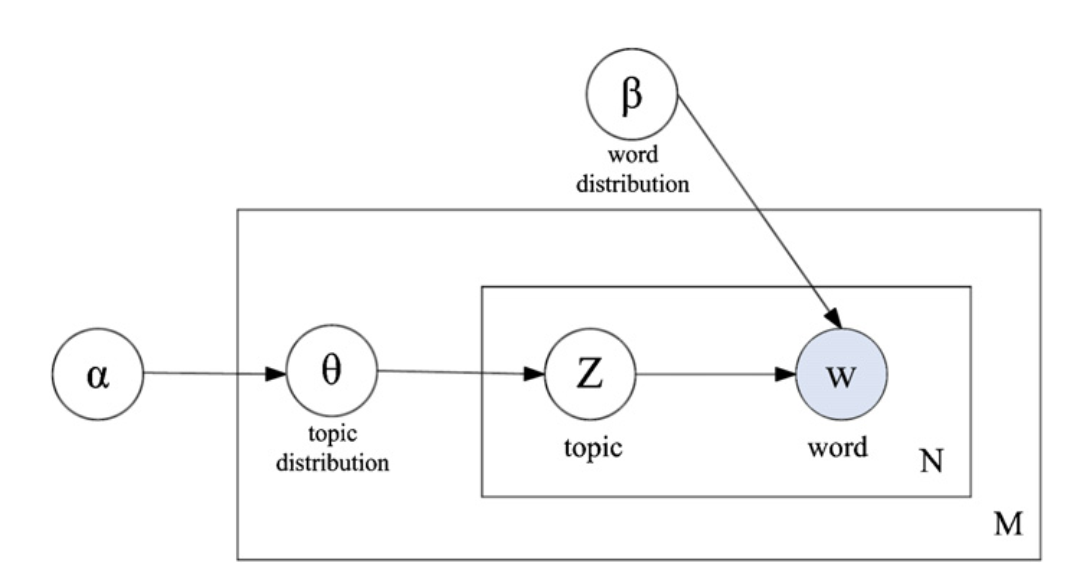
\includegraphics[scale=0.4]{../Figure/cao_juan.PNG}
    \caption{Schematic representation of Latent Dirichlet Allocation}
    \end{centering}
    \begin{footnotesize} 
        \begin{center}
            \textbf{Adapted from \citeA{cao2009density}.}
        \end{center}
    \end{footnotesize}
\end{figure}

    \section{Data}
    We used Pushshift’s Reddit dataset \cite{baumgartner2020pushshift} to investigate our research questions. This dataset is a data-dump of all submissions and comments on Reddit from 2005 to December 2019. We limited our scope to include two of the largest subreddits concerning smart home technologies: “homeautomation” (approx. 1 million members) and “smarthome” (approx. 91 k members). We included data from July 2017 - December 2019. This resulted in 379.883 individual text elements of submissions and comments. 

To avoid bots, we took an ensemble approach with both manual and automatic screening of posts. The manual screening was simply based on whether “bot” was a part of the username. A total of 40 accounts were identified as being bots. During this manual screening it was found that many bots explicitly stated that they were indeed bots. This led us to the simple idea of automatically screening users based on a regex expression designed to capture all posts in which “I am a bot” or variations thereof were present. Besides this, it has been found \cite{skowronski_identifying_2019} that the best predictor of a user being a bot is the similarity of their posts. In an accurate ML model this single feature accounted for more than 46\% of the decision weight \cite{skowronski_identifying_2019}. In short, bots generally tend to post either identical or similarly worded comments. We automatically excluded users with posts that were more than 40% identical to each other according to the SequenceMatcher from the difflib python library. These two automatic screening processes resulted in the exclusion of 44 accounts, ultimately leading to the exclusion of 84 accounts. 

    \subsection{Preprocessing}
    We removed stopwords from the text using nltk’s \cite{loper2002nltk} stopwords as well as our own list of extended stopwords. We also removed submissions and comments where 70\% of words were not in nltk’s list of english words. Finally, we used spacy’s \cite{spacy2} english language model to get the lemma for each word . 

As Reddit comments often consist of very few words, it makes sense to exploit the hierarchical structure of posts to create documents that consist of several comments that relate to each other. For RQ1 we are interested in simply squeezing as much information as possible out of the discussions on the Reddit forums. We were unsure as to whether it would be easier for LDA models to group the Reddit discussion into interpretable topics based on either (1) documents based on all comments relating directly to each other or (2) documents based on all comments to a post. We call the first case “trees” and the second case “threads”. In the “tree” approach the implicit assumption is that the comments on Reddit posts diverge and constitute distinct discussions. In the “thread” approach all comments to a post are included in a single document that is fed to the LDA model, and as such the implicit assumption is that all comments to a post will be around a single topic. In addition to finding the best unit of analysis, modelling the data based on two ways of grouping the data should allow us to draw more robust conclusions. 
For RQ2 we decided to only include text from the user submitting the original post in the documents fed to the LDA. We call this “submissions” and use this as we are interested in whether users initialize a conversation about the three query words “trust”, “security” and “privacy”, and not how these are used more generally in the comments of posts. As “submissions” only include posts and comments made by the original authors, we believe this to be an efficient way of shaping the data to our interests. In sum this results in three different “atomic” units that we investigate in parallel and make different LDA models for (see Fig. 1). The concatenation of text into these groups resulted in Submissions consisting of 52115 documents, Threads consisting of 52115 documents and Trees consisting of 196667 documents. 

\begin{figure}[H]
    \begin{centering}
    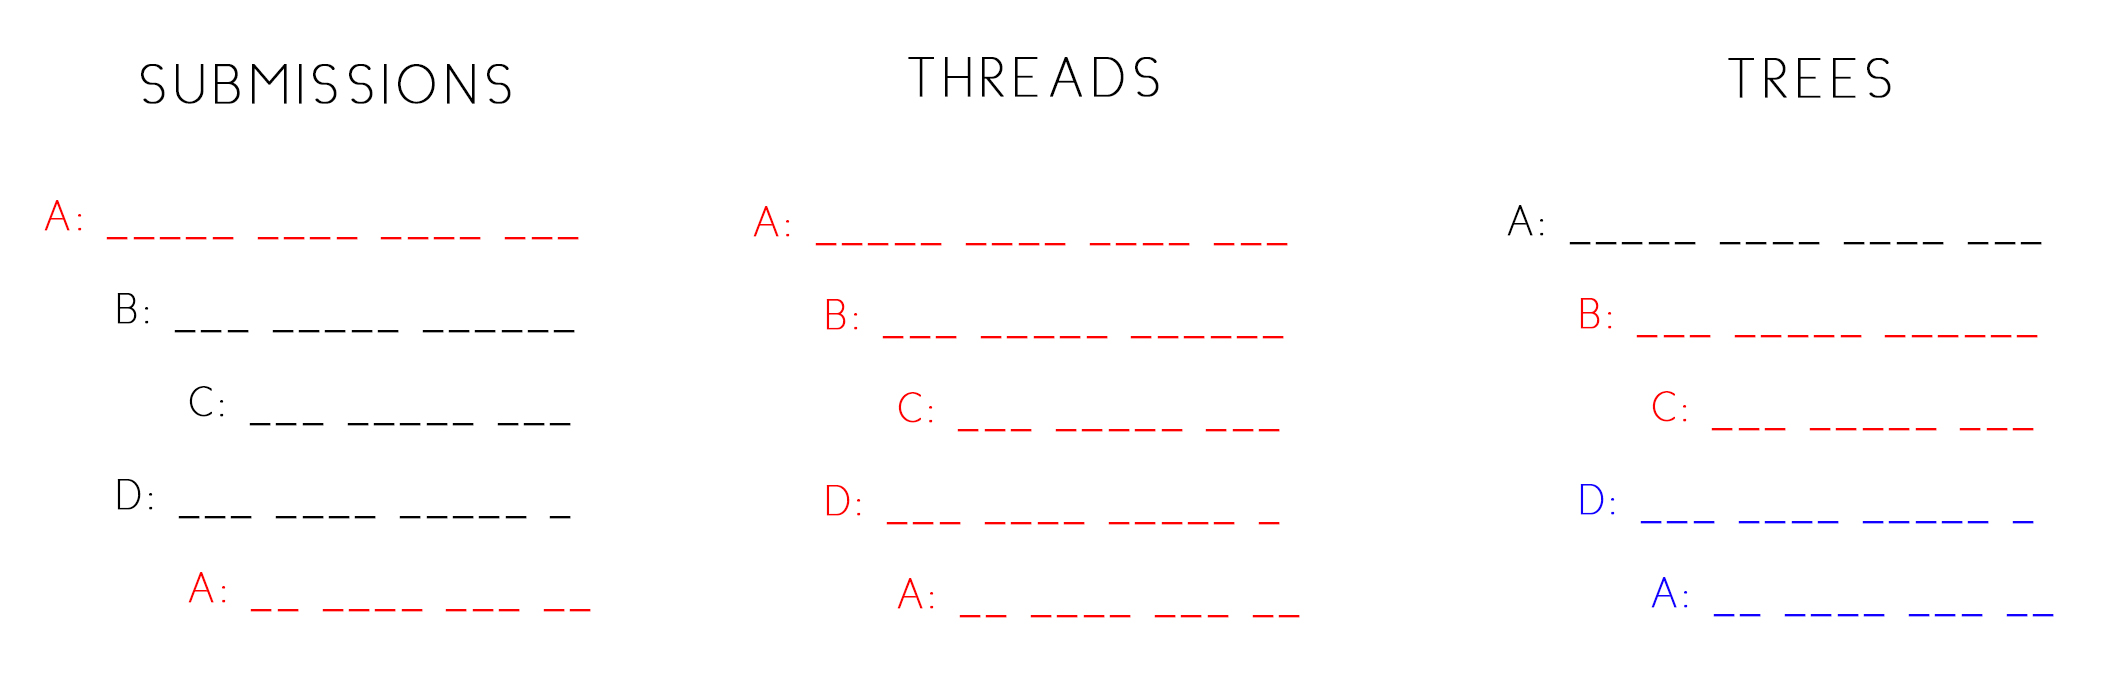
\includegraphics[scale=0.45]{../Figure/atomic_units.jpg}
    \caption{Atomic units of analysis}
    \end{centering}
    \begin{footnotesize} 
        Atomic units of analysis. Submissions are generated by only considering the original post and the comments from the author of the post. Threads concatenate the original post and all the comments into one document. Finally, Trees keeps some of the inherent hierarchical structure from the post. This is done by splitting posts into different documents, by splitting for each first tier comment and all the comments to this comment. Importantly, the text from the original post is pasted into all trees of a post.
    \end{footnotesize}
\end{figure}

We followed many of methodological choices made in prior work regarding preprocessing. Our main addition to the preprocessing pipeline is optimizing running time and making a flexible system, which enables the extraction of all these different atomic units effortlessly. As we are increasing the amount of data substantially (from 5000 to 196667 documents in the biggest corpus), run time becomes essential. The previous framework was not geared to handle this amount of data. As an example, we optimized the lemmatization process, cutting run time from roughly $\sim$43 hours to around $\sim$2 hours. 

By enabling efficient parsing of the data into different atomic units, we easily compute and compare results obtained by models trained on different data. More importantly, this allows us to have different datasets for our first and second research question. 

    \section{Methods}
    \subsection{Topic Modelling}
    As has been mentioned a key methodology for both RQ1 and RQ2 is topic modeling using LDA. There are many options available, two of the most popular python implementations being Gensim’s implementation (Radim, 2010) and the Mallet wrapper (McCallum, 2002) for Gensim. Gensim uses a Variational Bayes sampling method while the Mallet wrapper uses Gibbs sampling. Generally, Gensims implementation is faster, while Mallet’s Gibbs sampling method has been found to be more precise (Rafferty, 2019). In the process of our work we tried both approaches but did not find evidence that Mallet was more precise. Because of this we used the Gensim implementation run on multiple CPU cores to optimize run time. A note is that Gensim does not appear to support GPU processing, and although the multicore implementation does positively affect run time, the models (especially “trees”) take a long time to run. 
Another nice thing about Gensim is that the $\alpha$, $\beta$ and $k$ hyperparameters can be easily tweaked by the user from within python. After running into issues with automatically learning assymetric priors for the $\alpha$ and $\beta$-parameter (Radim, 2010), we chose to do a grid search over all combinations of plausible candidate values for the hyperparameters. Because of demanding run times we limited the grid to the following values for both threads and trees (RQ1) and submissions (RQ2): 
\begin{align*} 
    \alpha&: 0.01,\; 0.1,\; 1\\
    \beta&: 0.01, \; 0.1, \; 1 \\
    k&: 5, \; 10, \; \ldots,\; 50     
\end{align*}

The values chosen for $\alpha$ and $\beta$ are chosen to jump in powers instead of linearly as this ensures that the grid searches a more balanced and wide space. The values for these two parameters should be reasonable since $\alpha = 1$ and $beta = 1$ are uniform distributions, while $\alpha < 1$ is a symmetric distribution which assumes that documents are composed of few topics and $\beta < 1$ is a symmetric distribution which assumes that topics are comprised of few words. Generally, $\alpha$ and $\beta$ below 1 are reasonable for natural language because of sparsity. 
We run the Gensim multicore LDA model with the number of passes set to 10 and chunksize set to 2000. These appear to be reasonably common values. The chunksize is the number of documents processed before the model updates and the number of passes is the number of times that the LDA model goes through the whole corpus of documents.

    \subsection{Different Metrics to evaluate Quality of Topics}
There are several ways of finding a good topic model. Because topic models, such as LDA are generative, a typical assessment has been to use predictive accuracy such as held-out likelihood and perplexity \cite{chang2009reading}. However, these evaluations do not directly address human interpretability of topics, which is the goal here. In fact, \citeA{chang2009reading} report an overall negative correlation between these validation metrics and human interpretability. In large part due to \citeA{chang2009reading}, coherence measures have been developed for topic models (including LDA). Topic coherence measures how often topic words appear together in a corpus and is a good proxy for human interpretability (Konstantinovskiy, 2016). The baseline implementation in Gensim’s model evaluation “c\_v coherence” is used here as a quantitative measure of how our LDA models are. c\_v coherence is bounded in the [0, 1] range, with larger values being better. 
An issue with coherence measures however, is that they tend to continue improving for a larger number of topics, which we also see in our case (see fig. x below). Human interpretability of topics on the other hand typically does not keep improving for a larger number of topics \cite{chang2009reading}. To address this issue we used additional evaluation metrics from \citeA{cao2009density} and \citeA{arun2010finding} and based our model selection on an ensemble approach. Both \citeA{cao2009density} and \citeA{arun2010finding} focus specifically on finding the right number of topics (k) rather than on optimizing other hyperparameters such as ($\alpha$, $\beta$). \citeA{cao2009density} presents a measure based on topic distribution over words. The intuition is that the right amount of topics (k) will be the amount of topics where words are generally associated with as few topics as possible. The average cosine distance is used to assess the correlation between topics, which should be as small as possible and is experimentally validated \cite{cao2009density}. The measure presented in \citeA{arun2010finding} is technically pretty involved, and an explanation for the mathematics will not be provided here. The main point for our purposes is that \citeA{arun2010finding} presents empirical evidence that for the right number of topics (k) the measure hits a minimum. We did not develop any rigorous method for combining the values of the three measures (c\_v coherence, \cite{cao2009density}, \cite{arun2010finding}) and as such we based our selection of reasonable $\alpha$, $\beta$ and $k$ on eye-balling (see Fig. x below). 
It should be noted that we do not interpret the absolute values of these evaluation metrics but rely on the relative difference between all of our models' performance against these metrics to find good candidates. 

\begin{figure}[H]
    \begin{centering}
    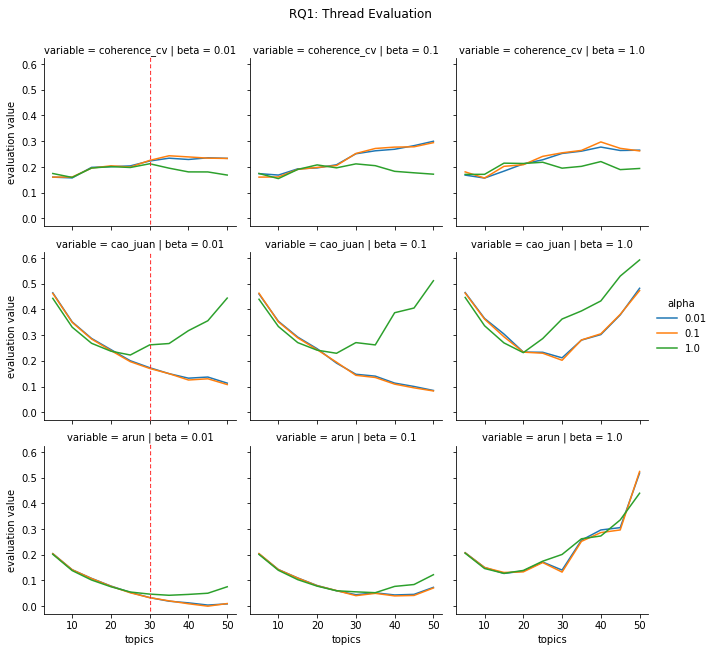
\includegraphics[scale=0.4]{../Figure/H1_thread_red.png}
    \caption{Evaluation of Topic Models (Threads)}
    \end{centering}
    \begin{footnotesize} 
        Grid search of Topic Models over 50 topics with Thread as atomic unit. Red dashed shows the selected amount of topics. 
    \end{footnotesize}
\end{figure}

The previously described quantitative metrics for model quality are valuable in that they help us narrow the search space of candidate models. Because we created LDA models for three different subsets of our dataset (threads, trees, submissions) and ran over a fairly large grid, it was practically impossible to visually inspect all of the models. However, the whole purpose of conducting LDA was in our case to interpret the topics and gain an exploratory overview of the themes discussed on the Reddit forums. As such, the next step was to visually inspect the models. This was done primarily using pyLDAvis and word clouds \cite{sievert2014ldavis}. 
Eventually we settled on interpreting LDA models with $k = 30$, $\alpha$ = 0.01 and $\beta$ = 0.01 for both submissions (RQ2) as well as threads and trees (RQ1). These models performed quantitatively reasonable (see plot above and appendix). More importantly however, the topics were found to be generally more interpretable and useful than for larger or smaller values for the $k$ parameter. As such, all results from here on out will be from models with these parameters. 

    \subsection{Labeling based on Hubert et al. (2020)}
    As mentioned previously, \citeA{hubert2020take} provides a list of key terms that cover the categories of smart home devices. In order to structure the bottom-up LDA topics we attempted to label the topics into his six categories. These are “home entertainment” (e.g. smart speakers), “control and connectivity” (e.g. smart assistants), “security” (e.g. camera, windows), “comfort and lighting” (e.g. bulbs), “energy management” (e.g. thermostats) and “smart appliances” (e.g. smart fridges) \cite[p. 1]{hubert2020take}. Beyond the categories listed in \citeA{hubert2020take}, we include two categories; “random” and “misc”. The random category covers topics that are not semantically coherent or simply consist of a bunch of common words. The misc category covers topics that are interpretable and have semantically related words, but which do not appear to fit neatly into the categories of \citeA{hubert2020take}.  
    
    \subsection{Investigating "privacy", "trust" and "security"}
    To investigate how the three keywords “privacy”, “trust” and “security” are used on the two subreddits, we start by simply calculating the frequency of the words in the documents. This is done to get a first indication of whether these are frequently used words on the forums. After this screening, we find the most dominant topic of each document given our model. We examine topics which include the three words of interest as part of the ten highest weighted words. We then find the 10 documents that are deemed to be the most dominated by the given topic by the model while also including the word of interest. These 10 documents are then qualitatively assessed to estimate whether the documents are related to concerns regarding the users data. 
    \section{Results}
    \subsection{RQ1}
    FOR FIGURE 1: Our task in the first part of this paper was to gain an overview of the topics discussed in the Reddit forums “homeautomation” and “smarthome”. The central results can be summarized in three figures highlighting different aspects of the discussion of Smarthome applications on Reddit. Figure x. shows the prevalence of topics that we labelled as belonging to either of our eight categories, for the three atomic units that we worked with (RQ1: thread and tree, RQ2: submissions). Topic prevalence was calculated by finding the most dominant topic for each document, concatenating these topics into our predefined categories and calculating the relative frequency for each category. In general it is clear that the topics that cover Smarthome appliances according to \citeA{hubert2020take} are not equally represented in the discussion. Across the models from all different atomic units, “comfort and lighting”, “control and connectivity” and “security” are very prevalent. By contrast “smart appliances”, “home entertainment” and “energy management” are consistently marginal topics. The topic labels “misc” and “random” vary more. 
    
    \begin{figure}[H]
        \begin{centering}
        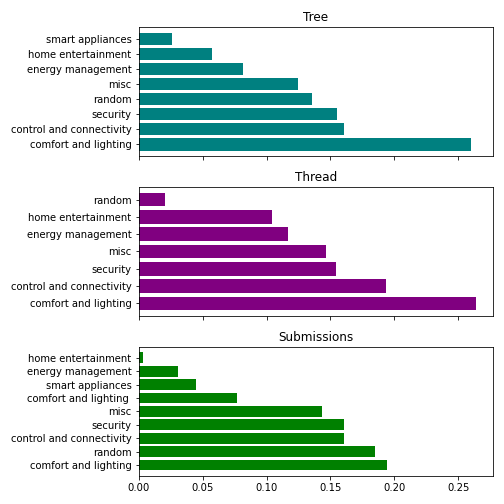
\includegraphics[scale=0.5]{../Figure/Topic_Prevalence.png}
        \caption{Category prevalence across different atomic units}
        \end{centering}
        \begin{footnotesize} 
            Category prevalence for all three atomic units. X-axis is relative contribution of each topic. 
        \end{footnotesize}
    \end{figure}
    
    FOR FIGURE 2: 
    We were interested to see whether the labels that we imposed on the topics corresponded to the bottom-up clustering of topics as generated by pyLDAvis using Jensen-Shannon distance \cite{sievert2014ldavis}. The three topics that were found to be prevalent across models, “comfort and lighting”, “control and connectivity” and “security” are also the ones that we see clustered in the figure below. The clusters that we have marked on the plot are not perfectly exclusive, in that they only include topics that we have labelled “comfort and lighting”, “control and connectivity” and “security” but it is very close. Easily close enough to suggest that the superimposed categories are good candidates for natural separators. The principal components themselves are extremely difficult to interpret and this will not be attempted here. For an interactive view of the plot, click \href{https://tinyurl.com/y9ncgo5b}{here}.
    
    \begin{figure}[H]
        \begin{centering}
        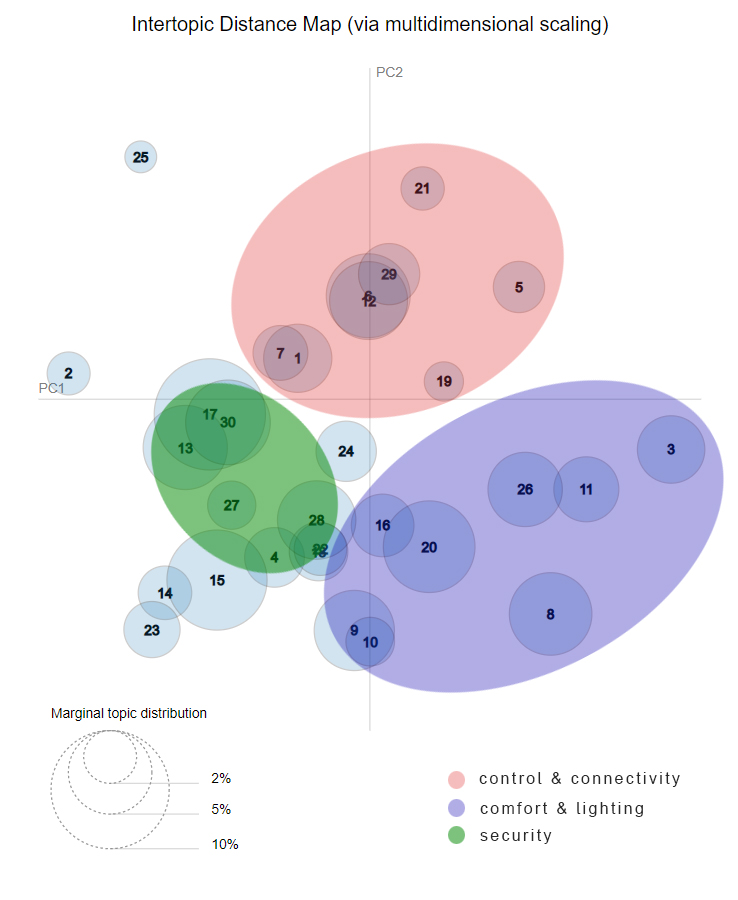
\includegraphics[scale=0.4]{../Figure/pyLDAvis_edit.jpg}
        \caption{pyLDAvis plot of the atomic unit Trees}
        \end{centering}
        \begin{footnotesize} 
            pyLDAvis plot of topics from LDA model on the atomic unit of Tree. Distances between topics calculated using Jensen-Shannon divergence \cite{sievert2014ldavis}. Using our own labels for each topic, rough boundaries between the three largest topics are colored. For more detail, the interactive plot is available \href{https://tinyurl.com/y9ncgo5b}{here}.
        \end{footnotesize}
    \end{figure}
    
    FOR FIGURE 3: 
The pyLDAvis plot above shows that the largest superimposed categories actually do occupy different parts in the model-space. However to really provide a full picture of the topics discussed we must investigate the miscellaneous (misc) category, which is the most prevalent category in RQ1 models besides the three big ones mentioned previously. A word-cloud plot of the top 50 terms in each topic labelled by us as “misc” is shown below. There might be an indication that topic 2, topic 17 and topic 25 are related to purchasing items and support. These three topics are also neighbors towards the upper-left quadrant of the pyLDAvis plot above. In addition topic 24 and 28 are neighbors in the middle of the pyLDAvis plot and seem to be related to a concrete sense of the “control and connectivity” topic. This topic could perhaps be partialled up into a more abstract and “smart” topic consisting of actual smart assistants and a more concrete one with key-words such as router, network and phone. 

\begin{figure}[H]
    \begin{centering}
    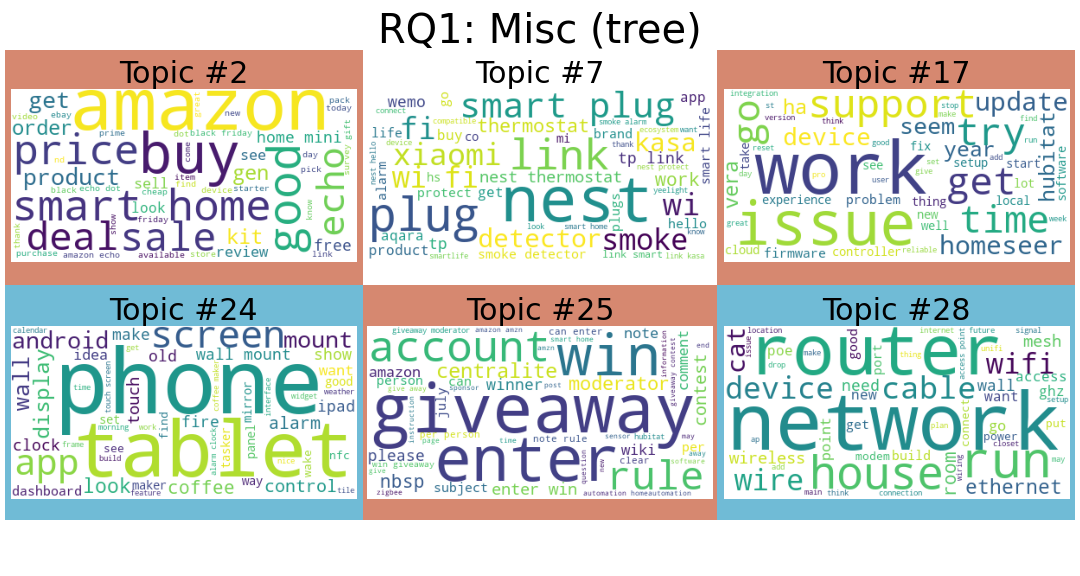
\includegraphics[scale=0.3]{../Figure/tree_misc_red.png}
    \caption{Word clouds of topics in the misc category}
    \end{centering}
    \begin{footnotesize} 
        showing word-clouds of the topics that we labelled as miscellaneous (misc) from RQ1 tree model with $\alpha = 0.01$, $\beta = 0.01$, $k = 30$. Colors indicate possible category relationships, where orange is related to purchasing items and support, while blue is related to concrete senses of connectivity. 
    \end{footnotesize}
\end{figure}

    \subsection{RQ2}
    By tracking the three query words “privacy”, “trust” and “security”, we find that they occur in 258, 333 and 2803 submissions respectively out of 52115 documents. These values correspond to 0.50\% of documents containing “privacy”, 0.64\% containing “trust” and 5.38\% containing “security”. 

    As almost no documents contained “privacy” and “trust” we investigated individual documents using these terms to assess the quality of the search terms. The content of these samples do seem to be revolving around the user’s privacy concerns regarding their data.
    
    Turning to the much more prevalent “security” key term. We first plotted the two topics which have the term “security” among the 10 highest weighted words. This shows that security is used alongside terms such as “soor”, “house” and “camera” (see fig. x below).
    
    \begin{figure}[H]
        \begin{centering}
        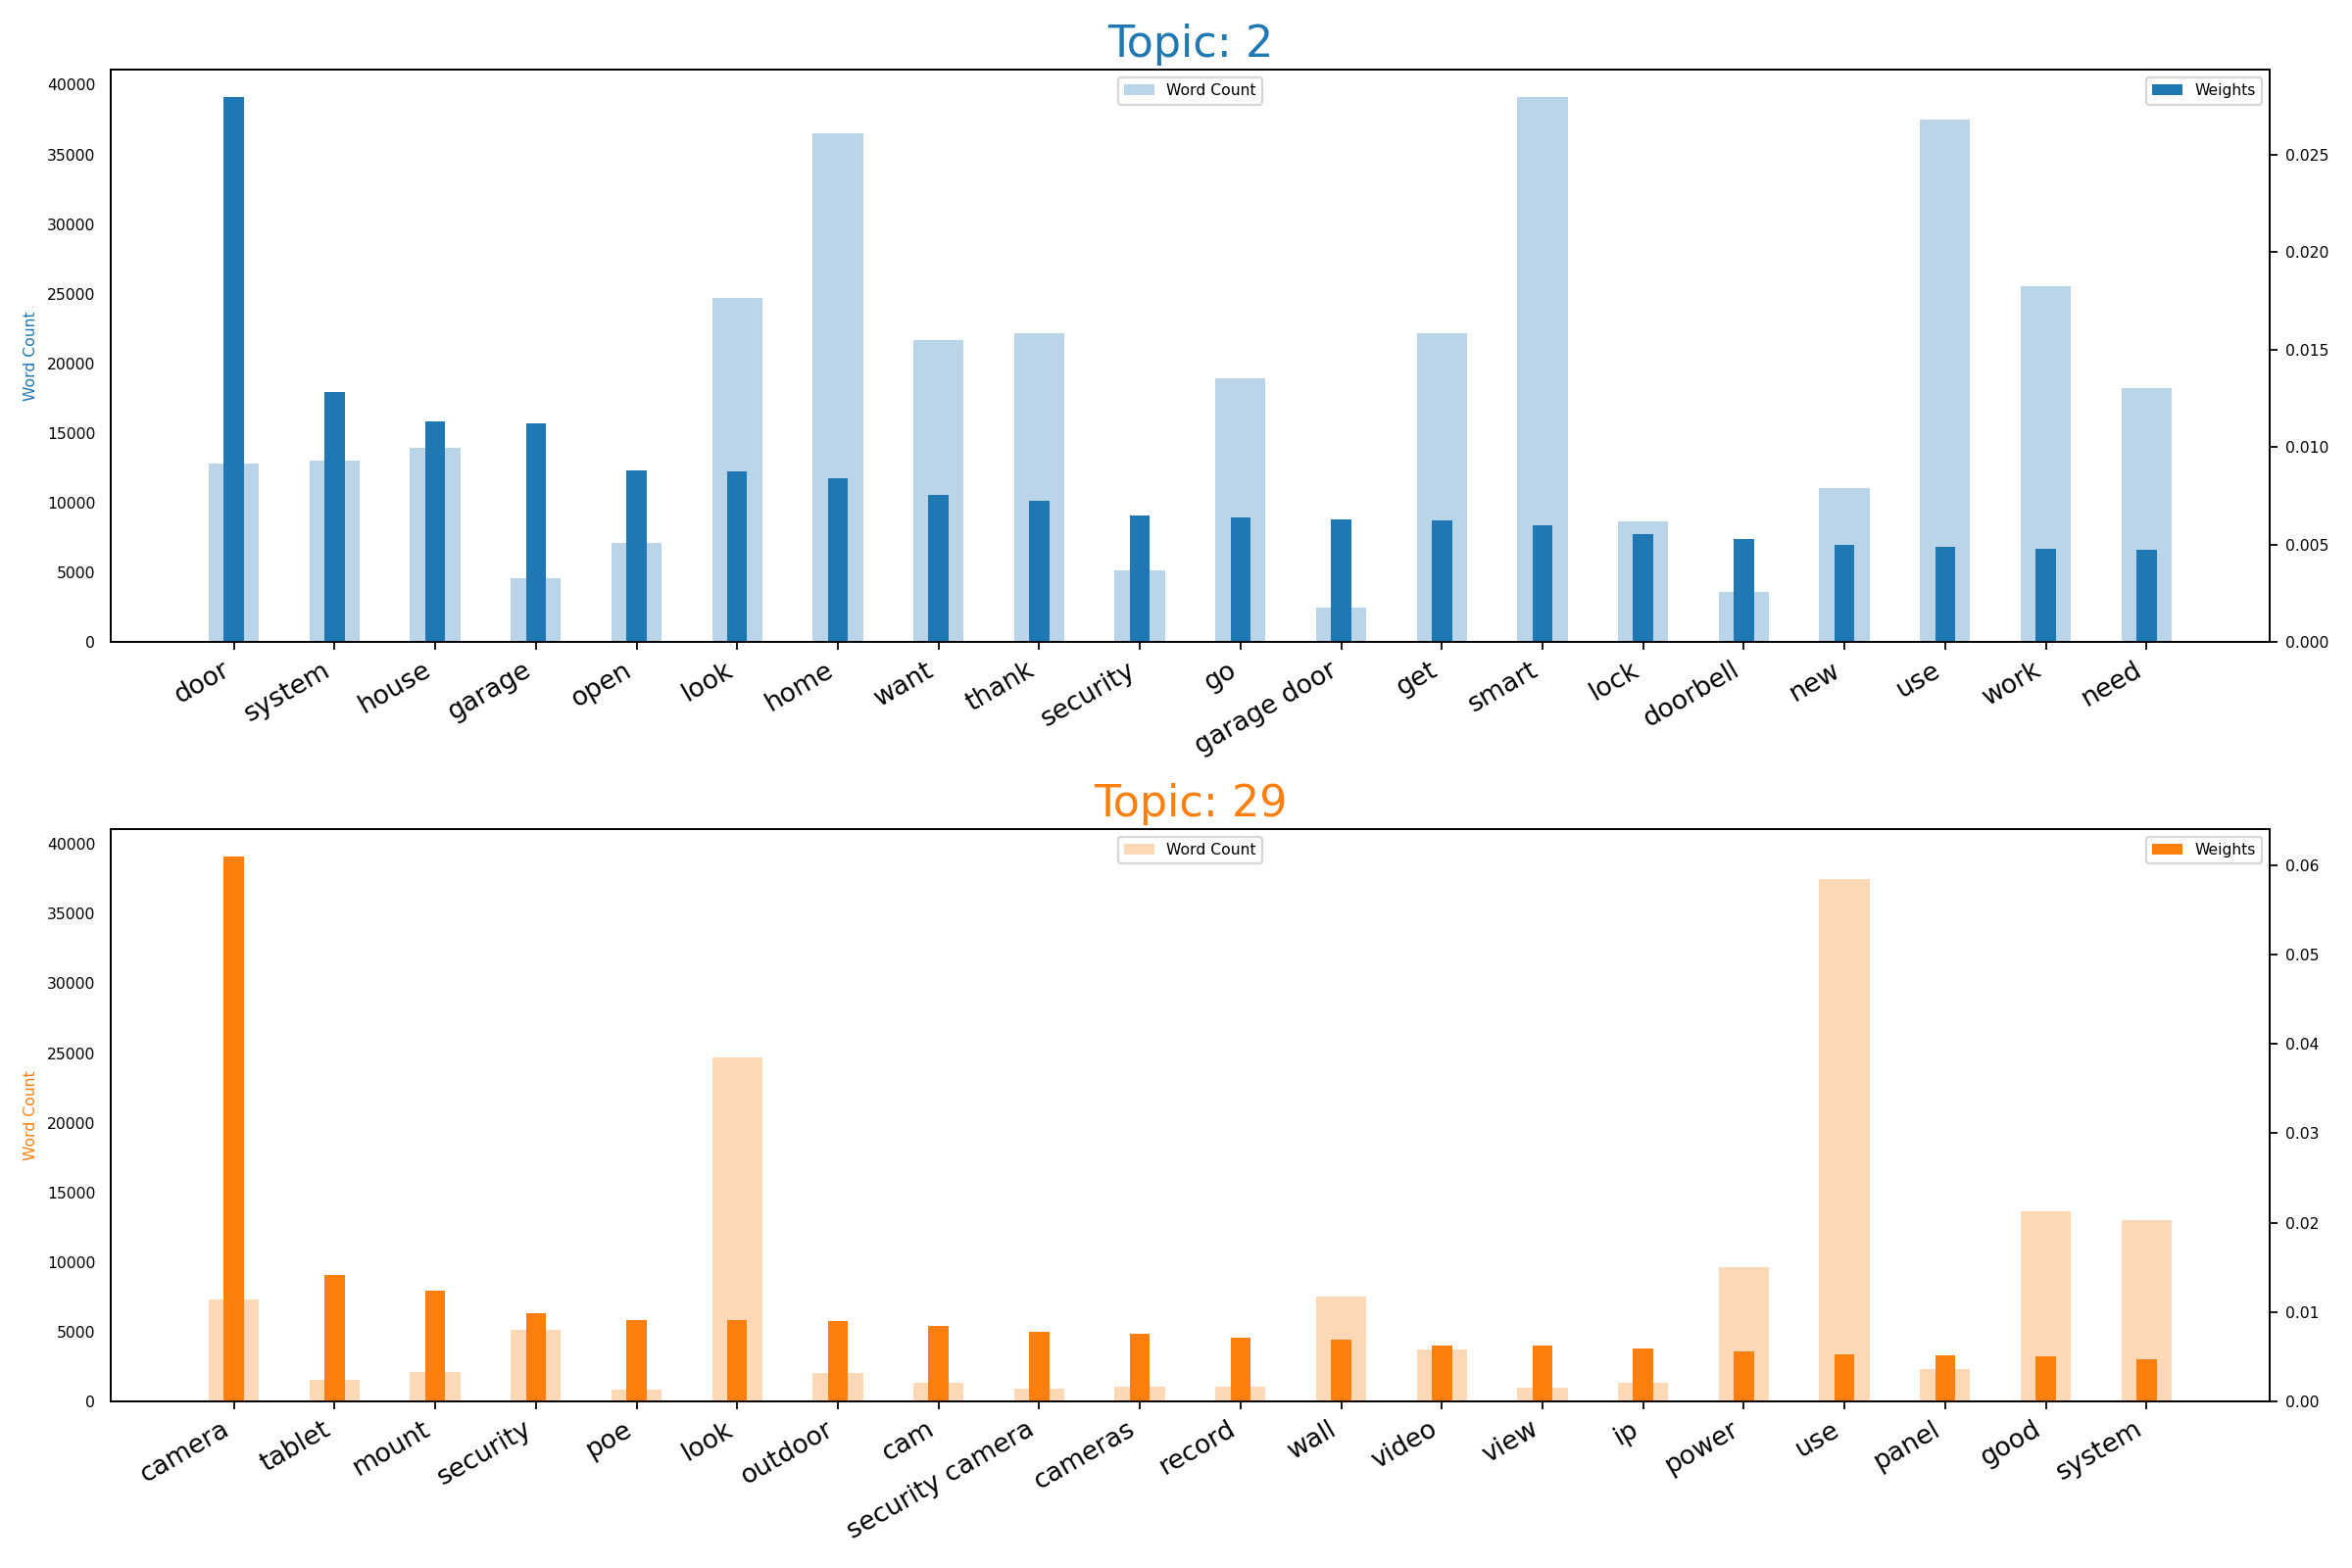
\includegraphics[scale=0.3]{../Figure/H2_topic_weight_prelim.png}
        \caption{Weights and frequency of top 10 words in topics concerning security}
        \end{centering}
        \begin{footnotesize} 
            Visualizing word counts and weights for Topic 2 and Topic 29 from the Submission Topic Model. Topics were chosen as they are the only two topics which have security as one of the ten words with the highest weights in the model. Left y-axis and opaque bars are word counts, and right y-axis and solid bars are weights of the model. 
        \end{footnotesize}
    \end{figure}

    We extracted submissions that were grouped into topics 2 and 29 and contained the key-word “security” to qualitatively assess whether these referred to security in a concrete sense (e.g. security cameras or locks) or an abstract sense (e.g. data security). The extracted submissions were found to use “security” in an overwhelmingly concrete sense (e.g. security cameras and locks) (see appendix). 

    \section{Discussion}
    \subsection{RQ2}
    Based on the low frequency of the words “privacy” and “trust” in the dataset, there seems to be little evidence that concerns over the privacy of one's data is a central discussion on the subreddits. The search terms did in fact match documents in which “privacy” and “trust” were used to mean what we had expected, and such the most natural conclusion seems to be the discussion around privacy and trust is marginal on these forums. 
Security is the only query word which is used regularly. This is both in terms of raw frequency, and as an important word in the topics from our topic models. This could suggest that many users are concerned with either data security (e.g. co-occurring with “data” and “surveillance”) or that users are generally concerned with house security (e.g. “security” co-occurring with “house”, “camera” and “lock”). We do in fact find the latter. It seems to us as though the abstract (data) sense of “security” is semantically more related to the terms “privacy” and “trust” and the apparent marginal usage of security in this sense converges with the finding that “privacy” and “trust” are rarely used to clearly indicate that this is not a central topic of discussion. 
This finding is surprising to us, since this concern over privacy and data security is generally thought to be major parts of the debate around smart home technologies \cite{hubert2020take,tabassum2019investigating}. However, the finding that these are not in fact major topics of debate does seem to agree with the finding of \cite{hubert2020take} that “privacy” and “trust” were not significant mediators of smart home. 

    \subsection{RQ1}
    The topics found in the topic models correspond well with the predefined categories defined by \citeA{hubert2020take}. It is important to note that we do find indications that the topics do not appear at the same frequencies at all. Our results indicate that categories, such as “smart appliances” are very rarely talked about on the subreddits. In comparison, “comfort and lighting” are discussed to a large extent. In sum, we find that these different categories should not be considered equally in terms of frequency in the discussion of smart home users.
From comparing the topics found in all three topic models, there also seems to be indications that the results seem to generalize across atomic units. This should bolster our belief that the resulting topics are robust and prevalent in the discussion. This is especially the case, as we labelled the categories prior to visualizing and inspecting them. 

We do however also find topics, which fall outside these predefined categories, but were meaningful; the “misc” category. Recall, that we mentioned purchasing as well as practical connectivity as possible relations between some of the topics found in the “misc” category. However, there is also a common denominator between purchasing relation and the practical connectivity relation. Whether it be buying the next device or setting up the connections for it, these are concrete actions. In fact, most topics revolve around concrete products and problems - not abstract discussions. 

    \subsection{The Forum}
    To us the results from our investigation of both RQ1 and RQ2 suggests that the Reddit forum is overwhelmingly practically oriented rather than oriented towards abstract discussions. This is eminently clear from the finding that “privacy”, “trust” and the abstract notion of “security” are extremely rare. However, it also seems clear from the LDA topics from RQ1, many of which seem to revolve around specific types of smart home products and many of which are very low-tech, centering around cables, prices and hue. Based on our results, such as “which light should I buy?”, “has anyone tried this smart speaker?” should be more common than questions such as “should I be concerned about my privacy when talking around Alexa?”. 

This begs the question of whether smart home users are generally unconcerned with notions of privacy and security surrounding personal data, or whether that is simply not what is primarily discussed on these specific subreddits. It might be the case that genuine users of smart home technologies are simply okay with trading privacy for functionality \cite{hubert2020take, tabassum2019investigating}. However, it might also be that the discussion on other forums (e.g. Twitter) is different and focuses more on notions of privacy surrounding personal data. In that case it would seem that RQ2 is not best pursued using this dataset. 

    \section{Future work}
    \subsection{Reddit as a practical forum}
    Based on our investigation we are not in a position to tell whether smart home users are generally unconcerned with privacy regarding data security, or whether this topic of discussion is marginal specifically in the investigated subreddits. By analyzing data across different discussion boards from different websites (e.g. Twitter), one could investigate whether the observations that we have observed generalize. If the analysis shows that (a) the words “privacy” and “trust” are consistently underrepresented in the corpus and (b) that topics indicate that security is largely linked to a more concrete sense of security, we would have stronger evidence for the claim that smart home users in general are either (a) unconcerned with privacy of data or (b) that they have accepted the trade-off between functionality and supplying personal data. 
    \section{Conclusion}
    Using LDA as our main methodology we investigated the discussions on two of the biggest subreddits concerning smart home technologies. We find that topics generally tend to fall in previously proposed categories, but that “control and connectivity”, “comfort and lighting” and “security” dominate the discussion. Using three query words of interest (“trust”, “privacy”, “security”) we sought to estimate the degree to which users were concerned about data security issues. We find that “trust” and “privacy” are used in less than 1\% of documents. Moreover, when security is used, it is used to refer to security systems or security cameras, not the security of one’s data. We are not in a position to conclude whether users of smart home technologies are generally unconcerned about data security, or whether the subreddits are simply not used to discuss these issues. We therefore suggest that future research should include additional discussion boards from other sites (e.g. Twitter) to investigate whether the apparent lack of concern regarding data security and privacy is a general feature of the community of smart home technology users, or simply an idiosyncratic property of the forum. In this regard, our efforts to make the pipeline easily reproducible and flexible could help make future efforts easier to conduct. 

    \section{Appendix}
    \begin{figure}[H]
        \begin{centering}
        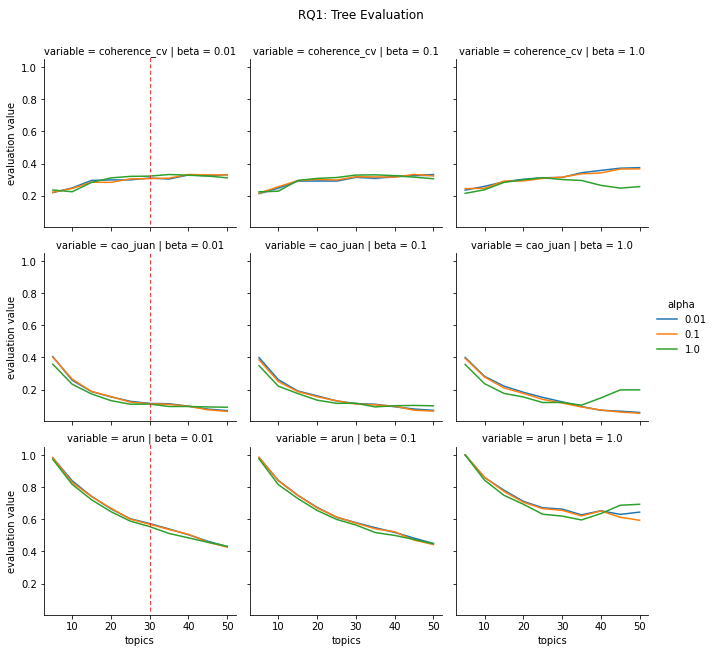
\includegraphics[scale=0.4]{../Figure/H1_tree_red.png}
        \caption{Evaluation of Topic Models (Trees)}
        \end{centering}
        \begin{footnotesize} 
            Grid search of Topic Models over 50 topics with Tree as atomic unit. Red dashed shows the selected amount of topics.         \end{footnotesize}
    \end{figure}

    \begin{figure}[H]
        \begin{centering}
        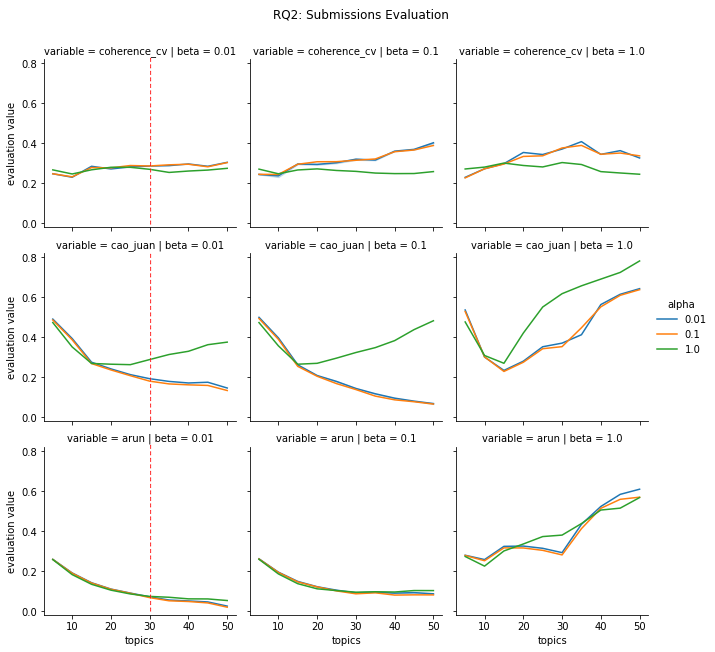
\includegraphics[scale=0.4]{../Figure/H2_submissions_red.png}
        \caption{Evaluation of Topic Models (Submissions)}
        \end{centering}
        \begin{footnotesize} 
            Grid search of Topic Models over 50 topics with Submission as atomic unit. Red dashed shows the selected amount of topics.  
        \end{footnotesize}
    \end{figure}

    \bibliographystyle{apacite}

    \bibliography{cite}
\end{document}